\textit{\chapter{Diseño e implementación}} % Main chapter title

\label{Chapter3} % Change X to a consecutive number; for referencing this chapter elsewhere, use \ref{ChapterX}

\definecolor{mygreen}{rgb}{0,0.6,0}
\definecolor{mygray}{rgb}{0.5,0.5,0.5}
\definecolor{mymauve}{rgb}{0.58,0,0.82}

%%%%%%%%%%%%%%%%%%%%%%%%%%%%%%%%%%%%%%%%%%%%%%%%%%%%%%%%%%%%%%%%%%%%%%%%%%%%%
% parámetros para configurar el formato del código en los entornos lstlisting
%%%%%%%%%%%%%%%%%%%%%%%%%%%%%%%%%%%%%%%%%%%%%%%%%%%%%%%%%%%%%%%%%%%%%%%%%%%%%
\lstset{ %
  backgroundcolor=\color{white},   % choose the background color; you must add \usepackage{color} or \usepackage{xcolor}
  basicstyle=\footnotesize,        % the size of the fonts that are used for the code
  breakatwhitespace=false,         % sets if automatic breaks should only happen at whitespace
  breaklines=true,                 % sets automatic line breaking
  captionpos=b,                    % sets the caption-position to bottom
  commentstyle=\color{mygreen},    % comment style
  deletekeywords={...},            % if you want to delete keywords from the given language
  %escapeinside={\%*}{*)},          % if you want to add LaTeX within your code
  %extendedchars=true,              % lets you use non-ASCII characters; for 8-bits encodings only, does not work with UTF-8
  %frame=single,	                % adds a frame around the code
  keepspaces=true,                 % keeps spaces in text, useful for keeping indentation of code (possibly needs columns=flexible)
  keywordstyle=\color{blue},       % keyword style
  language=[ANSI]C,                % the language of the code
  %otherkeywords={*,...},           % if you want to add more keywords to the set
  numbers=left,                    % where to put the line-numbers; possible values are (none, left, right)
  numbersep=5pt,                   % how far the line-numbers are from the code
  numberstyle=\tiny\color{mygray}, % the style that is used for the line-numbers
  rulecolor=\color{black},         % if not set, the frame-color may be changed on line-breaks within not-black text (e.g. comments (green here))
  showspaces=false,                % show spaces everywhere adding particular underscores; it overrides 'showstringspaces'
  showstringspaces=false,          % underline spaces within strings only
  showtabs=false,                  % show tabs within strings adding particular underscores
  stepnumber=1,                    % the step between two line-numbers. If it's 1, each line will be numbered
  stringstyle=\color{mymauve},     % string literal style
  tabsize=2,	                   % sets default tabsize to 2 spaces
  title=\lstname,                  % show the filename of files included with \lstinputlisting; also try caption instead of title
  morecomment=[s]{/*}{*/}
}

En este capítulo se presentan las características de diseño y desarrollo de todos los componentes que forman parte del sistema, descritos en el capítulo 2.

%----------------------------------------------------------------------------------------
%	SECTION 1
%----------------------------------------------------------------------------------------
\section{Arquitectura del sistema}

En la figura 3.1 se presenta el diagrama general del sistema.

\begin{figure}[H]
	\centering
	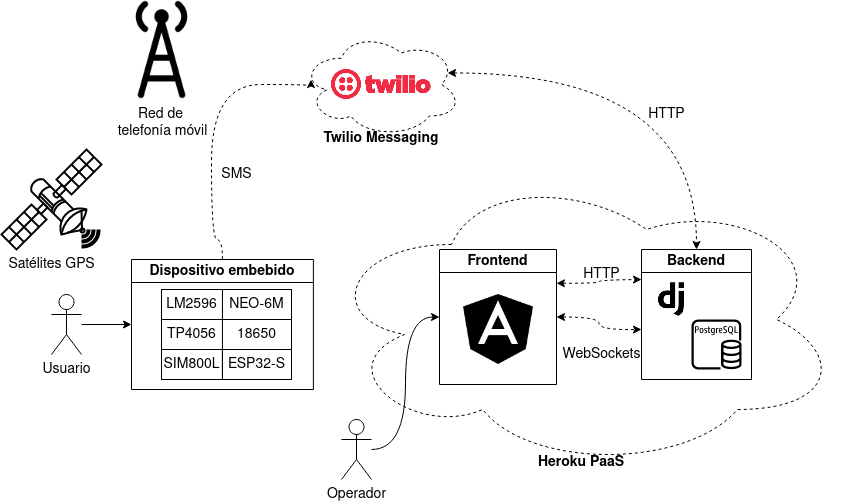
\includegraphics[width=1\textwidth]{./Figures/arquitectura.png}
	\caption{Arquitectura general del sistema.}
	\label{fig:texmaker}
\end{figure}


Se pueden identificar los siguientes componentes dentro de la arquitectura desarrollada:
\begin{itemize}
	\item En primer lugar, se observa a un usuario del dispositivo embebido, que es el componente que envía alertas mediante SMS hacia el servicio de mensajería en la nube.
	\item En segundo lugar, se encuentra la plataforma de Twilio, que recepciona los mensajes recibidos y los reenvía mediante un \textit{webhook} hacia el servicio web o \textit{backend}. La comunicación entre el dispositivo embebido y Twilio fue posible ya que en este último se contrató un número teléfonico para la recepción de los SMS. 
	\item En tercer lugar, el \textit{backend}, que es el componente encargado de la recepción de alertas, procesamiento y almacenamiento de datos y comunicación con el \textit{frontend}. Fue desarrollado con el framework Django en Python.
	\item A continuación, se ubica el \textit{frontend}, que es la aplicación web que se encarga de toda la interacción del usuario operador con el sistema, incluyendo carga de datos y gestión de alertas. Consiste en una \textit{Single Page Application } y su desarrollo fue realizado en Angular, cuyo lenguaje es TypeScript \citep{ANGULAR:1}.
	\item Por último, se encuentra un componente menor, pero no menos importante que es la base de datos encargada de almacenar toda la información del sistema, como usuarios, alertas, tipos de alertas, entre otros. El motor elegido fue PostgreSQL.
\end{itemize}

Todos los \textit{servicios} del \textit{backend} requieren de autenticación y autorización por parte del operador, a excepción de algunos que deben ser públicos para ser utilizados.
   
\section{Desarrollo de módulos de hardware}

El firmware del dispositivo embebido fue desarrollado con el \textit{Espressif IoT Development Framework}, conocido como ESP-IDF, el framework oficial de la placa de desarrollo elegida para el proyecto, ESP32-S \citep{ESPIDF:1}. Su lenguaje de programación es C y provee un robusto conjunto de bibliotecas para el desarrollo sobre periféricos y funcionalidades del ESP32. Adicionalmente, ESP-IDF funciona como registro de un conjunto de componentes realizados por el fabricante oficial o la comunidad para extender funcionalidades comunes de los sistemas embebidos. 

El firmware se desarrolló para una placa ESP32-WROOM-32 del fabricante NodeMCU, que conforma un kit atractivo por su bajo costo, interoperabilidad, documentación disponible y bajo consumo de energía. La ventaja de usar esta placa es que además de contar con el framework ESP-IDF y todas las características descritas en el capítulo 2, permite que el firmware desarrollado pueda ser adaptado y reutilizado para otras placas de características similares.

Por otra parte, se importaron varias bibliotecas usadas para el desarrollo embebido. Entre estas, resulta interesante destacar dos bibliotecas importantes:
\begin{itemize}
	\item \textit{libnmea}: biblioteca que facilita la lectura de los datos recibidos del módulo GPS \citep{LIBNMEA:1}. Esto es posible ya que el NEO-6M utiliza un formato de mensajes estándar denominado NMEA \citep{NMEA:1}. La ventaja de usar \textit{libnmea} es que convierte los datos recibidos en estructuras de C, lo que permite acceder rápidamente a valores como la latitud, longitud, etc.
	\item \textit{iot-button}: biblioteca que permite configuraciones complejas sobre botones o pulsadores \citep{BUTTON:1}. La ventaja de utilizar este componente es que permite rápidamente configurar funciones de \textit{callback} ante eventos como pulsaciones largas, sin requerir que se desarrolle lógica de control, así como también contempla solución ante inconvenientes como un \textit{debounce} o falsas pulsaciones al momento de accionar el botón \citep{DEBOUNCE:1}.
\end{itemize}

Estas dos bibliotecas fueron importadas al proyecto como \textit{managed components}, propios del registro de componentes externos de ESP-IDF \citep{ESPIDF:1}. En la tabla \ref{tab:bibliotecas-esp32} se encuentra detallado el uso que tuvo cada biblioteca utilizada para el firmware.

\begin{table}[H]
	\centering
	\caption[Bibliotecas más relevantes utilizadas.]{Bibliotecas más relevantes utilizadas.}
	\begin{tabular}{l c}    
		\toprule
		\textbf{Bibilioteca} & \textbf{Uso} \\
		\midrule
		\makecell[l]{\textit{iot\_button.h}} & \makecell{Implementación del botón pulsador y acciones \\ a tomar al momento de ser usado. } 	\\
		\hline
		\makecell[l]{\textit{nmea.h}}	 & \makecell{Lectura de mensajes NMEA recibidos por el módulo \\ GPS.} 	\\		
		\hline
		\makecell[l]{\textit{string.c}}  & \makecell{Manipulación y transformación de cadenas de texto \\ al momento de leer mensajes recibidos de los módulos.}  \\
		\hline	
		\makecell[l]{\textit{ctype.c}}  & \makecell{Uso de funciones comunes de C \\ para trabajar sobre caracteres de texto. }  \\
		\hline
		\makecell[l]{\textit{uart.h}}	 & \makecell{Comunicación con los módulos GSM y GPS \\ mediante puerto serie.}	\\
		\hline	
		\makecell[l]{\textit{esp\_system.h}} &  Funciones básicas del ESP-IDF.\\
		\hline
		\makecell[l]{\textit{esp\_log.h}} &  \makecell{Visualización de errores y mensajes de \textit{debug} \\ del firmware.} \\
		\hline
		\makecell[l]{\textit{esp\_pm.h} \\ \textit{esp\_sleep.h}} & Configuraciones de ahorro de energía. \\
		\hline
		\makecell[l]{\textit{adc\_oneshot.h} \\ \textit{adc/adc\_cali.h} \\ \textit{adc\_cali\_scheme.h}}  & \makecell{Conversión analógico-digital y lectura de \\ valores para calcular la carga de la batería.} \\
		\hline
		\makecell[l]{\textit{nvs.h} \\ \textit{nvs\_flash.h}} &  \makecell{Manejo del almacenamiento \textit{flash} para \\ guardar datos en la memoria no volátil.} \\
		\hline
		\makecell[l]{\textit{freertos/FreeRTOS.h}} & \makecell{Configuración del sistema operativo en tiempo real  \\ del ESP32.} \\
		\hline
		\makecell[l]{\textit{freertos/task.h}} & Implementación de funciones como procesos/tareas. \\
		
		\bottomrule
		\hline
	\end{tabular}
	\label{tab:bibliotecas-esp32}
\end{table}

Para el desarrollo, compilación, pruebas y monitoreo, se trabajó con el entorno integrado Visual Studio Code en conjunto con la extensión oficial de ESP-IDF. Esta última facilita el trabajo con el kit de desarrollo y la incorporación y uso de módulos propios del ecosistema del ESP32. En la figura \ref{fig:esp32:diagrama} se pueden observar los componentes físicos del dispositivo embebido.


\begin{figure}[H]
	\centering
	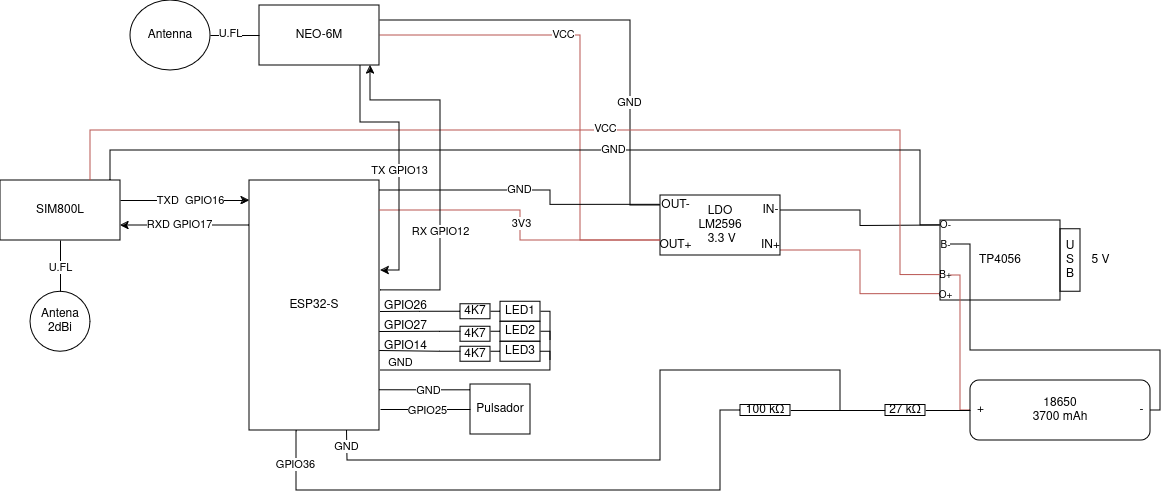
\includegraphics[width=0.95\textwidth]{./Figures/esp32-arquitectura.png}
	\caption{Esquema de componentes de hardware del dispositivo embebido.}
	\label{fig:esp32:diagrama}
\end{figure}

\pagebreak

Adicionalmente, se incorporó un regulador de tensión LM2596 en la entrada de energía de la batería, que permite adecuar el voltaje de entrada de 4,2 V a 3,3 V \citep{LM2596:1}, requeridos por el ESP32 y el NEO-6M. Además, se añadió una antena activa para el módulo GPS ya que con una antena pasiva la precisión de la localización obtenida era baja o tomaba más tiempo del esperado adquirir buena señal. Por otra parte, se reemplazó la antena helicoidal del módulo GSM por una con formato PCB y 3 dBi de ganancia.


\subsection{Tareas del dispositivo embebido}

Para implementar las funciones del dispositivo embebido, se dividió el desarrollo del firmware en 7 bloques o funciones de código principales. Estas se pueden describir de la siguiente forma:

\begin{itemize}
	\item Inicio: consiste en la función de arranque del firmware, en donde se realizan acciones como inicialización de periféricos, revisión de errores de arranque, reducción de la velocidad de reloj del procesador al mínimo requerido, asignación inicial de variables y por último, la configuración de las tareas que corren en bucle. Posterior al inicio, esta función finaliza su ejecución. En la figura \ref{fig:esp32:tasks1} se pueden observar todos los pasos contemplados. No es una tarea en el sentido estricto de \textit{FreeRTOS}.
	\item Manejador del módulo GSM: consiste en una función con un bucle infinito que lee el puerto serie cada pocos segundos para detectar comandos/respuestas del módulo GSM y tomar una acción ante cada mensaje si corresponde. En la figura \ref{fig:esp32:tasks1} se puede visualizar el bucle con las acciones que realiza. Los mensajes recibidos que se gestionan son:
		\begin{itemize}
			\item \texttt{AT}: mensaje que representa un OK.
			\item \texttt{CMT}: mensaje que significa que se recibió un SMS; esto se utiliza para configurar el número de teléfono al cual se le deben enviar las alertas por SMS.
			\item \texttt{CMGS}: mensaje que significa que se envió correctamente un SMS; se utiliza para confirmar el envío correcto de una alerta.
			\item \texttt{CSQ}: mensaje que informa el nivel de calidad de la señal de telefonía móvil.
			\item \texttt{GSN}: mensaje que informa el IMEI del dispositivo; se utiliza como mecanismo de seguridad ya que el SMS de configuración de teléfono debe incorporar los primeros dígitos del IMEI como validación.		
		\end{itemize}
		\item Manejador del módulo GPS: consiste en una función con un bucle que se encarga de recibir comandos/respuestas del módulo GSM leyendo el puerto serie y de guardar la información recibida. Existen diferentes tipos de mensajes, pero para los fines del registro de la localización, solamente se está guardado la información del tipo de mensaje \textit{GPGGA}, que indica la posición actual y datos de los satélites \citep{NMEA:2}. En la figura \ref{fig:esp32:tasks1} se puede visualizar el bucle con las operaciones.
		\begin{figure}[H]
	\centering
	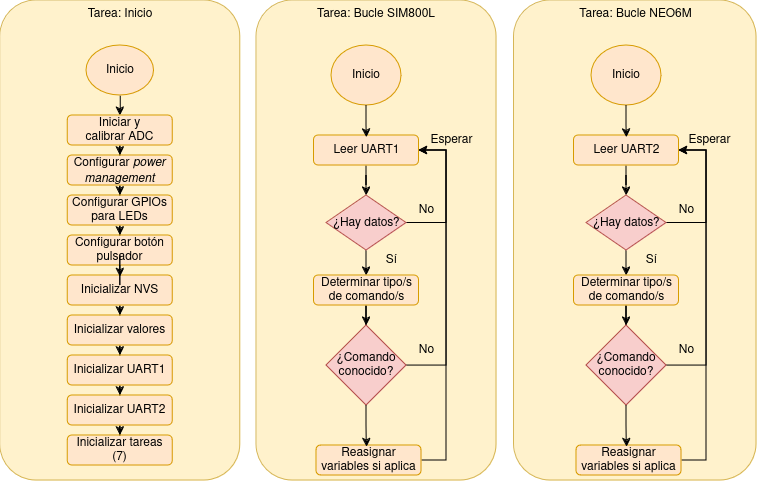
\includegraphics[width=0.95\textwidth]{./Figures/esp32-tasks1.png}
	\caption{Diagramas de flujo de tarea inicial y bucles del módulo GSM y GPS.}
	\label{fig:esp32:tasks1}
\end{figure}
		\item \textit{Setup} de energía del módulo GSM: tarea que espera por la correcta inicialización del módulo GSM y posteriormente aplica algunas optimizaciones de energía. En la figura \ref{fig:esp32:tasks2} se listan los pasos efectuados. Luego, la tarea termina su ejecución.
		\item \textit{Setup} de energía del módulo GPS: tarea que espera por la inicialización del módulo GPS y comunicación con al menos 5 satélites para enviarle algunos comandos de optimización. Luego de esto, la tarea finaliza. En la figura \ref{fig:esp32:tasks2} se pueden visualizar el flujo de esta.
		\begin{figure}[H]
	\centering
	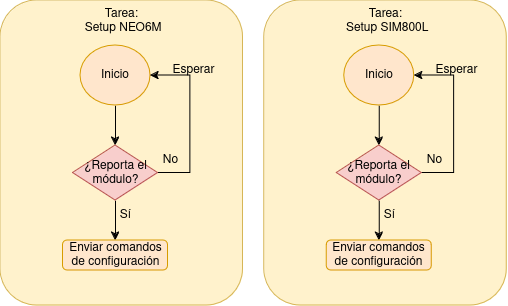
\includegraphics[width=0.75\textwidth]{./Figures/esp32-tasks2.png}
	\caption{Diagramas de flujo de las tareas de \textit{setup} de energía.}
	\label{fig:esp32:tasks2}
\end{figure}

		\item Control de estado de GPS, GSM y batería: esta tarea tiene como objetivo cada 30 segundos, leer el estado de las variables de calidad de la señal GSM, determinar la cantidad de satélites conectados y nivel de batería, y parpadear 3 luces dependiendo del estado de estas variables. En el desarrollo, se repartió en tres funciones pequeñas, pero a fines explicativos se presenta como una única tarea. En la figura \ref{fig:esp32:tasks3} se puede observar el flujo de ejecución de la tarea.
		\item Almacenamiento periódico de datos: cada 1 minuto esta tarea se encarga de leer las variables de latitud, longitud, IMEI y número de teléfono asignado y almacenarlas en el almacenamiento no volátil en el caso de que los valores fueran válidos. En la figura \ref{fig:esp32:tasks3} se puede observar el bucle ejecutado por la tarea.
		\item Control periódico del módulo GSM: esta tarea se encarga de solicitarle información al módulo GSM sobre el estado de la red cada 1 minuto. Esto es debido a que el módulo GSM no reporta automáticamente su estado, a diferencia del módulo GPS que sí lo hace.  En la figura \ref{fig:esp32:tasks3} se puede apreciar el control que realiza la función.
		
	\begin{figure}[H]
		\centering
		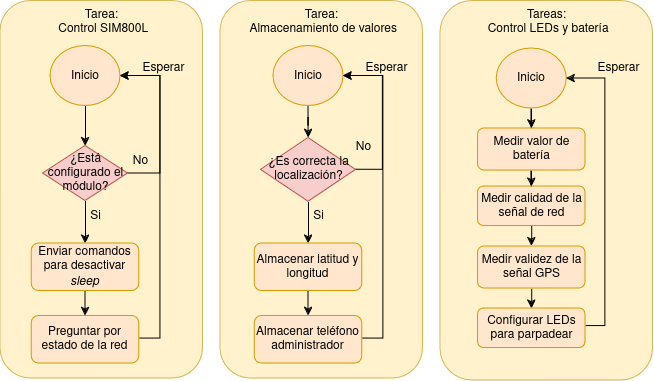
\includegraphics[width=0.9\textwidth]{./Figures/esp32-tasks3.png}
		\caption{Diagramas de flujo de las tareas de control y almacenamiento.}
		\label{fig:esp32:tasks3}
	\end{figure}

\end{itemize}

Para finalizar, se puede considerar una última función más dentro del firmware que es el interruptor ante la pulsación del botón activador. En caso que se supere un umbral de 3 segundos del pulsador presionado, se activará un \textit{callback} definido para ese evento. Este se encarga de levantar los valores actuales de la última localización válida almacenada, de determinar cual es el número de teléfono al cual se debe enviar el mensaje de alerta y emitir los comandos hacia el módulo GSM para enviar el SMS. 

En la figura \ref{fig:esp32:callback-codigo} se muestra un diagrama de flujo resumido de la interrupción. Para la asociación del \textit{callback} con el evento, se puede ver en el código \ref{esp32:callback-codigo} la implementación, donde \texttt{sos\_button\_long\_press\_cb} es una función definida y \texttt{cfg} es la definición del evento.

\pagebreak

\begin{lstlisting}[label=esp32:callback-codigo,caption=Definición del evento y asociación del \textit{callback}.]  % Start your code-block
// SOS button configure
button_config_t gpio_btn_cfg = {
    .type = BUTTON_TYPE_GPIO,
    .long_press_time = SOS_BUTTON_LONG_PRESS_TIME_MS,
    .gpio_button_config = {
        .gpio_num = SOS_BUTTON,
        .active_level = 1,
        .enable_power_save = true},
};

button_handle_t gpio_btn = iot_button_create(&gpio_btn_cfg);
if (NULL == gpio_btn)
{
    ESP_LOGE(TAG, "Button create failed");
}

button_event_config_t cfg = {
    .event = BUTTON_LONG_PRESS_START,
    .event_data.long_press.press_time = SOS_BUTTON_LONG_PRESS_TIME_MS,
};

ESP_ERROR_CHECK(iot_button_register_event_cb(gpio_btn, cfg, sos_button_long_press_cb, NULL));

\end{lstlisting}

\begin{figure}[H]
	\centering
	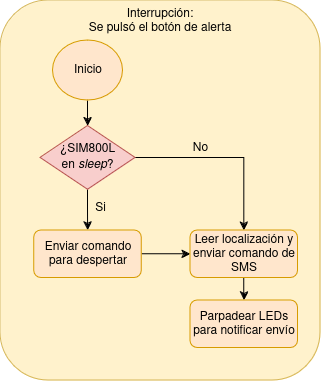
\includegraphics[width=0.5\textwidth]{./Figures/esp32-callback.png}
	\caption{Diagrama de flujo del \textit{callback} por pulsación.}
	\label{fig:esp32:callback-codigo}
\end{figure}


\subsection{Optimizaciones de energía aplicadas}

Se aplicaron diferentes técnicas de optimización sobre el ESP32 y los módulos GSM y GPS con el objetivo de optimizar y disminuir el consumo de energía:
\begin{itemize}
	\item Se configuró \textit{FreeRTOS} para solamente utilizar un núcleo del ESP32.
	\item Se limitó la frecuencia del procesador para solamente utilizar como máximo 80 MHz.
	\item Se desactivaron todos los periféricos no usados, como WiFi, Bluetooth, etc.
	\item Se configuró el \textit{Dynamic frequency scaling} o DFS del ESP32, que permite que se reduzca la velocidad del reloj del procesador de forma automática en determinadas condiciones \citep{ESP32:2}.
	\item Se configuró el modo \textit{sleep} del módulo SIM800L, desactivándolo solo cuando se le deben enviar comandos.
	\item Se desactivó el LED de notificación de calidad de señal del módulo SIM800L, ya que la comprobación se realiza de forma programática.
	\item Se redujo la frecuencia de actualización de mensajes del módulo NEO-6M hacia el ESP32.
	\item Se aplicó sobre NEO-6M una configuración de energía denominada \textit{Power Save Mode} para reducir la frecuencia de actualización hacia los satélites GPS \citep{NEO6M:2}.
	\item Se configuró el modo \textit{sleep} del módulo SIM800L, desactivándolo solamente cada ciertos intervalos de tiempo.
	\item Se utilizaron tiempos muertos de espera o \textit{standby} del orden de varios segundos en el ESP32, lo que resultó en que gran parte del tiempo la placa se encuentre en espera.
	\item Se redujo el consumo de energía de los 3 LEDs indicadores de GSM, GPS y batería mediante la incorporación de resistencias, lo que dio lugar a un consumo de aproximadamente 1 mA para todos los LEDs.
\end{itemize}

Además, se intentó aplicar un manejo tanto manual como automático (configurable mediante el uso de DFS) del modo \textit{light sleep} pero se encontró que, después de varios intentos y pruebas, el consumo de energía no disminuyó. Se interpretó, en base a las pruebas durante el desarrollo, que esto se debe a características de fabricación del modelo ESP32-WROOM-32 de NodeMCU. Se midió un consumo en \textit{idle} de aproximadamente 15 mA, aunque esté en \textit{deep sleep} o \textit{light sleep}.

\section{Desarrollo de módulo de \textit{backend}}

Para el desarrollo de la aplicación \textit{backend} y sus funcionalidades de API, se estructuró el proyecto siguiendo los lineamientos de Django, que consiste principalmente en dividir la aplicación en módulos web por temática o características. Para el caso de esta aplicación se identificaron dos módulos:
\begin{itemize}
	\item \textit{Users}: para englobar toda la funcionalidad referida a usuarios.
	\item \textit{Alerts}: para englobar toda la funcionalidad referida a beneficiarios/dispositivos y alertas.
\end{itemize}

Esto es una forma lógica de estructurar la información perteneciente a la misma lógica de negocio. En la figura \ref{backend:folder1} y \ref{backend:folder2} se pueden visualizar las carpetas de cada módulo con sus respectivos componentes.

\begin{figure}[H]
\centering
\begin{minipage}{.5\textwidth}
  \centering
  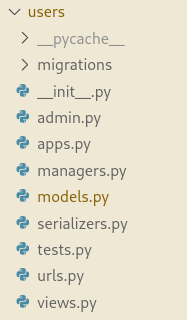
\includegraphics[width=.75\linewidth]{./Figures/backend-folder1.png}
  \captionof{figure}{Estructura de archivos de módulo de \textit{Users}.}
  \label{backend:folder1}
\end{minipage}%
\begin{minipage}{.5\textwidth}
  \centering
  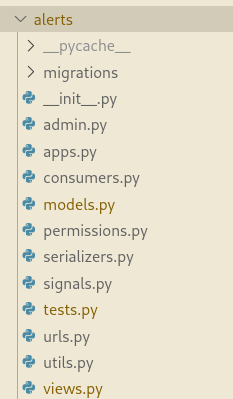
\includegraphics[width=.75\linewidth]{./Figures/backend-folder2.png}
  \captionof{figure}{Estructura de archivos de módulo de \textit{Alerts}.}
  \label{backend:folder2}
\end{minipage}
\end{figure}

Para la implementación se incorporaron varias bibliotecas externas, cuya utilidad se muestra en la tabla \ref{backend:libraries}:

\begin{table}[H]
	\centering
	\caption[Bibliotecas externas más relevantes.]{Bibliotecas externas más relevantes.}
	\begin{tabular}{l c}    
		\toprule
		\textbf{Bibilioteca} & \textbf{Uso} \\
		\midrule
		\makecell[l]{\textit{djangorestframework}}	 & \makecell{Biblioteca de Django para el \\ desarrollo de APIs REST.} 	\\		
		\hline
		\makecell[l]{\textit{psycopg}}  & \makecell{Biblioteca para conexión a \\ PostgreSQL \citep{DJANGO:4}.}  \\
		\hline	
		\makecell[l]{\textit{django-twilio}}  & \makecell{Biblioteca oficial \citep{DJANGO:3} de Twilio para \\ comunicación con \textit{Twilio Messaging Services}. }  \\
		\hline
		\makecell[l]{\textit{channels}}	 & \makecell{Biblioteca para la implementación de \\ WebSockets en Django \citep{DJANGO:5}.}	\\
		\hline	
		\makecell[l]{\textit{djangorestframework-simplejwt}} &  \makecell{Biblioteca para el \textit{middleware} de \\ autenticación de usuarios.} \\
		\hline
		\makecell[l]{\textit{drf\_yasg}} &  \makecell{Biblioteca para generar documentación \\ de API en Swagger.} \\
		\hline
		\makecell[l]{\textit{uvicorn}} & Servidor web ASGI para Python \citep{DJANGO:7}. \\
		\hline
		\makecell[l]{\textit{django-cors-headers}}  & \makecell{\textit{Middleware} de seguridad para peticiones \\ de la API.} \\
		\hline
		\makecell[l]{\textit{dj-database-url}} &  \makecell{Biblioteca para conectarse a base de datos \\ PostgreSQL de Heroku.} \\
		\hline
		\makecell[l]{\textit{django-channels-jwt}} & \makecell{\textit{Middleware} para autenticación \\ de WebSockets.} \\
		\bottomrule
		\hline
	\end{tabular}
	\label{backend:libraries}
\end{table}


En la figura \ref{backend:modulos} se presenta en forma de diagrama de bloques los principales componentes de la API:

\begin{figure}[H]
	\centering
	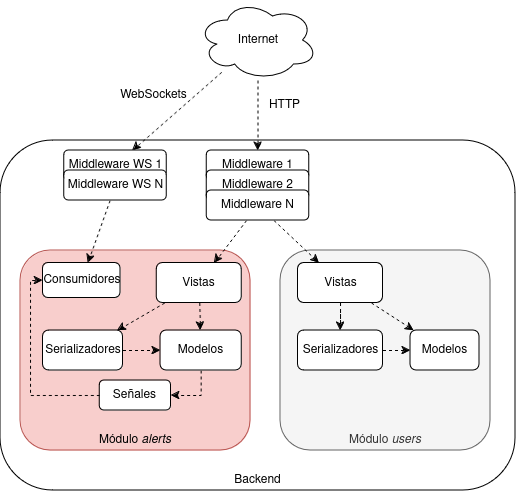
\includegraphics[width=0.9\textwidth]{./Figures/backend-componentes.png}
	\caption{Diagrama en bloques del \textit{backend}.}
	\label{backend:modulos}
\end{figure}

Se describen a continuación los componentes de mayor relevancia de los módulos:

\begin{itemize}
	\item Modelos: clases que representan los modelos de datos, como pueden ser las entidades de una alerta y un beneficiario.
	\item Serializadores: clases que agrupan la lectura, escritura, validación y salida de modelos de datos. Los serializadores permiten encapsular lógica de validación para diferentes operaciones o adaptar la representación de los datos según la necesidad \citep{DJANGO:8}. En el código \ref{backend:serializer1} se muestra el serializador de la entidad \textit{Beneficiary} junto con validaciones y acciones que deben realizarse durante la creación y actualización, así como también la definición de restricciones al momento de realizar la carga de datos.

\pagebreak

\begin{lstlisting}[language=Python,label=backend:serializer1,caption=Serializador de la entidad \textit{Beneficiary}.]  % Start your code-block

class BeneficiarySerializer(serializers.ModelSerializer):
    id = serializers.IntegerField(read_only=True)
    name = serializers.CharField(max_length=64, required=True)
    surname = serializers.CharField(max_length=64, required=True)
    telephone = serializers.CharField(
        max_length=32, required=True, validators=[only_int]
    )
    company = serializers.ChoiceField(
        choices=Beneficiary.COMPANY_CHOICES, default="OTH", required=False
    )
    enabled = serializers.BooleanField(default=True)
    type_id = serializers.IntegerField(allow_null=True, required=False)

    class Meta:
        model = Beneficiary
        fields = [
            ....
        ]

    def validate(self, data):
        ....

    def create(self, validated_data):
        ...

    def update(self, instance, validated_data):
        ....
\end{lstlisting}

	\item Vistas: clases que engloban peticiones HTTP sobre entidades o clases para atender un único tipo de petición, dependiendo del requerimiento \citep{DJANGO:9}. En el código \ref{backend:view1} se puede apreciar la definición del \textit{ViewSet} de la clase \textit{Beneficiary} y se observa que se asignaron de forma declarativa los permisos requeridos para realizar las peticiones y los filtros habilitados, sin requerir código adicional.
	
\begin{lstlisting}[language=Python,label=backend:view1,caption=\textit{ViewSet} de la entidad \textit{Beneficiary}.]  % Start your code-block

class BeneficiaryViewSet(EnablePartialUpdateMixin, viewsets.ModelViewSet):
    """
    A viewset that provides the standard actions for beneficiaries
    """

    permission_classes = [
        IsSameOrganization,
    ]
    serializer_class = BeneficiarySerializer
    filter_backends = [DjangoFilterBackend]
    filterset_fields = ["telephone", "name", "surname", "enabled"]

    def get_queryset(self):
        user = self.request.user
        queryset = self.filter_queryset(
            Beneficiary.objects.filter(organization=user.organization).order_by("id")
        )
        return queryset

    def destroy(self, request, *args, **kwargs):
        ....

    def update(self, request, *args, **kwargs):
        ....
\end{lstlisting}	
	
    \item Consumidores: representa un servicio de WebSockets que permite notificar en tiempo real una alerta nueva.
    \item \textit{Middlewares}: clases que permiten interceptar peticiones hacia la API \citep{DJANGO:10} y realizar comprobaciones como ver el rol del usuario o que este tenga la correcta autorización en las peticiones. No se desarrolló ningún \textit{middleware} sino que se incorporaron bibliotecas externas ya provistas.
    \item Señales: hace referencia a una notificación que se genera dentro de la aplicación ante un evento \citep{DJANGO:11}. En el marco de esta aplicación, cuando se almacena una nueva alerta se genera una señal que notifica al canal de \textit{WebSockets} que debe notificar el dato creado.
\end{itemize}

Respecto a las características del sistema, se lo diseñó con la idea de un producto \textit{multitenant}, es decir que permita que a futuro existan diferentes organizaciones cliente dentro de este \citep{DJANGO:12}. Debido a esta característica, todos los datos están contenidos dentro de una misma organización, compartida por los usuarios y beneficiarios, entre otros datos cargados. En la figura \ref{backend:modelo} se puede visualizar el modelo de datos relacional con las entidades diseñadas.

\begin{figure}[H]
	\centering
	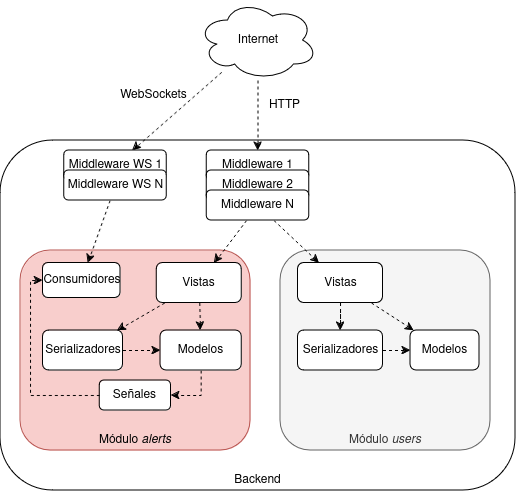
\includegraphics[width=0.75\textwidth]{./Figures/backend-modelos.png}
	\caption{Modelo de datos.}
	\label{backend:modelo}
\end{figure}


De todas maneras, para esta versión inicial solo se contempla un usuario por organización en el \textit{frontend}, aunque a futuro el diseño y la lógica de negocio en la API está diseñada para contemplar una organización con un usuario raíz o padre y un conjunto de usuarios operadores de menor privilegio.

\subsection{Servicios desarrollados}

A continuación, se muestran en la tabla \ref{tab:endpoints} los servicios implementados.

\begin{table}[H]
	\centering
	\caption[\textit{Endpoints} implementados.]{\textit{Endpoints} implementados.}
	\begin{tabular}{l c c}    
		\toprule
		\textbf{\textit{Endpoint}} 	 & \textbf{Descripción} \\
		\midrule
		GET /alert-types/ & Obtener tipos de alerta  \\		
		POST /alert-types/& Crear un tipo de alerta		\\		
		GET /alert-types/{id}/ & Obtener un tipo de alerta \\
		PUT /alert-types/{id}/ & Editar un tipo de alerta		\\
		DELETE /alert-types/{id}/ & Eliminar un tipo de alerta  \\
		\hline
		GET /alerts/ & Obtener alertas  \\		
		GET /alerts-summary/ & Obtener alertas de las últimas 24 horas \\		
		GET /alerts/{id}/ & Obtener una alerta \\
		PUT /alerts/{id}/ & Editar una alerta		\\
		PATCH /alerts/{id}/ & Editar parcialmente una alerta   \\
		\hline
		GET /beneficiaries/ & Obtener beneficiarios  \\			
		GET /beneficiaries/{id}/ & Obtener un beneficiario \\
		PUT /beneficiaries/{id}/ & Editar un beneficiario		\\
		PATCH /beneficiaries/{id}/ & Editar parcialmente un beneficiario   \\
		DELETE /beneficiaries/{id}/ & Desactivar un beneficiario \\
		\hline
		GET /beneficiary-types/ & Obtener tipos de beneficiarios  \\			
		GET /beneficiary-types/{id}/ & Obtener un tipo de beneficiario \\
		PUT /beneficiary-types/{id}/ & Editar un tipo de beneficiario		\\
		DELETE /beneficiary-types/{id}/ & Desactivar un beneficiario \\
		\hline
		POST /users/admin/ & \makecell{Crear un usuario administrador}  \\			
		GET /user-details/ & Obtener datos del usuario \\
		PATCH /user/{id}/ & Editar parcialmente un usuario \\
		\hline
		POST /login/ & Realizar login programático \\	
		GET /ws-auth/ & \makecell{Obtener token efímero para  conexión \\ a WebSockets} \\
		POST /twilio-webhook/ & \makecell{Webhook para notificar una  alerta \\ desde Twilio} \\	
		WS /ws/alerts/organization-{id}/ & Conectarse a canal de \textit{WebSockets}	\\
		\bottomrule
		\hline
	\end{tabular}
	\label{tab:endpoints}
\end{table}

Todos estos servicios fueron documentados mediante Swagger, una herramienta para documentación de APIs \citep{DJANGO:6}. Todas las vistas, a excepción del registro de un nuevo usuario administrador, requieren autenticación mediante un token. Esto es gestionado mediante la incorporación de un \textit{middleware} de Django, sin requerir código adicional más allá de declarar qué \textit{middlewares} utilizar para la autorización, como se observa en el código \ref{backend:settings1}.

\pagebreak

\begin{lstlisting}[language=Python,label=backend:settings1,caption=Configuración de \textit{middlewares} para la autenticación de la API.]  % Start your code-block

REST_FRAMEWORK = {
    "DEFAULT_SCHEMA_CLASS": "rest_framework.schemas.coreapi.AutoSchema",
    "DEFAULT_AUTHENTICATION_CLASSES": [
        "rest_framework_simplejwt.authentication.JWTAuthentication",
    ],
    "DEFAULT_PERMISSION_CLASSES": [
        "rest_framework.permissions.IsAuthenticated",
    ],
}

\end{lstlisting}

\section{Desarrollo de módulo de \textit{frontend}}

El desarrollo de la aplicación web en \textit{Angular} se estructuró siguiendo la convención estándar del framework \citep{ANGULAR:4}, como se puede apreciar en la figura \ref{frontend:folder}.

\begin{figure}[H]
	\centering
	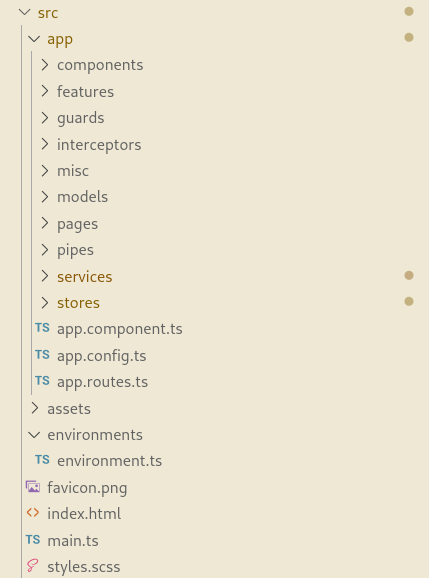
\includegraphics[width=0.5\textwidth]{./Figures/frontend-folder.png}
	\caption{Estructura del \textit{frontend}.}
	\label{frontend:folder}
\end{figure}

Respecto al uso de cada carpeta, se pueden describir las más relevantes de la aplicación:
\begin{itemize}
	\item \textit{pages}: corresponde a componentes que representan vistas enteras o secciones de la aplicación web.
	\item \textit{components}: corresponde a componentes invocados dentro de las páginas, como son los \textit{modals} o ventanas de carga de datos, el \textit{layout} o estructura base de la interfaz y otros componentes.
	\item \textit{stores}: hace referencia a clases que encapsulan datos y funcionan como una fuente de datos única para toda la aplicación \citep{NGRX:1}.
	\item \textit{services}: corresponde a clases que encapsulan el acceso a diferentes métodos del \textit{backend} para cada una de las entidades.
	\item \textit{models}: contiene la definición de interfaces para representar los modelos de datos.
	\item \textit{guards}: corresponde a clases que permiten limitar o no el acceso a una vista.
	\item \textit{interceptors}:	representa clases que interceptan llamadas HTTP y la comunicación de datos con el \textit{backend} para aplicar transformaciones de datos y redireccionar ante sucesos como errores.
	\item \textit{pipes}: clases que transforman la representación de objetos o datos hacia el usuario, como por ejemplo cambiar el formato de fecha y hora \citep{ANGULAR:5}.
\end{itemize}

En la figura \ref{frontend:esquema} se puede visualizar el diagrama en bloques del \textit{frontend}.
\begin{figure}[H]
	\centering
	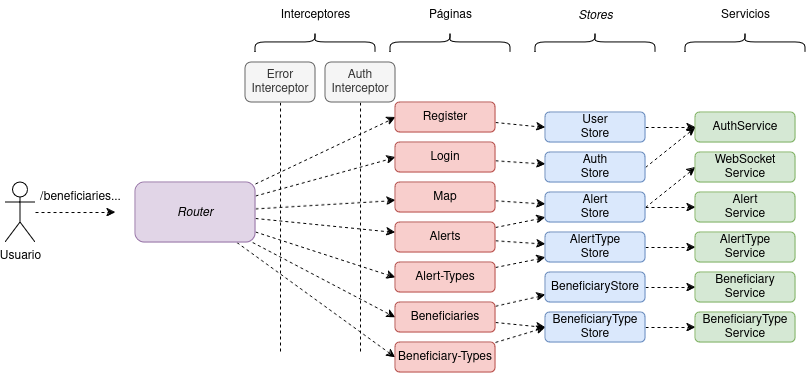
\includegraphics[width=0.95\textwidth]{./Figures/frontend-esquema.png}
	\caption{Diagrama en bloques del \textit{frontend}.}
	\label{frontend:esquema}
\end{figure}


La implementación de la estructura, el diseño de componentes y la visualización de formularios, entre otros componentes gráficos, contó con el uso de la biblioteca de estilos \textit{Angular Material} y con el uso de uno de los temas por defecto de la biblioteca. Toda la estructura se organizó solamente utilizando \textit{flexbox}, un método de diseño de páginas propio de \textit{CSS}, el lenguaje de estilos de los documentos web \citep{CSS:1}. No se contempló la necesidad de incorporar alguna herramienta o biblioteca para estructuras complejas, como por ejemplo \textit{Boostrap} que contiene un sistema de grilla \citep{BOOTSTRAP:1}, debido a que las páginas y secciones de la aplicación web son simples.

En relación a las páginas implementadas, se desarrollaron las rutas descritas en la tabla \ref{tab:frontend:pages}.

\begin{table}[H]
	\centering
	\caption[Rutas implementadas.]{Rutas implementadas.}
	\begin{tabular}{l c}    
		\toprule
		\textbf{Ruta} 	 & \textbf{Descripción} \\
		\midrule
		\textit{/login} & Sección de login  \\	
		\textit{/register} & Sección de registro de un nuevo usuario \\		
		\textit{/map} & Vista de mapa con las últimas alertas recibidas  \\
		\textit{/beneficiaries} & Listado de beneficiarios  \\	
		\textit{/beneficiary-types} & Listado de tipos de beneficiarios  \\		
		\textit{/alerts} & Listado de alertas  \\
		\textit{/alert-types} & Listado de tipos de alertas  \\
		\textit{/error} & Pantalla de error genérica  \\	
		\bottomrule
		\hline
	\end{tabular}
	\label{tab:frontend:pages}
\end{table}

\subsection{Particularidades del desarrollo}

En relación al manejo de datos desde la aplicación, se implementó en el \textit{frontend} un patrón de manejo de estado para las entidades del sistema denominado \textit{Store}, inspirado en patrones más complejos como \textit{Redux}, que surgieron para simplificar el manejo de estados en aplicaciones de usuario cada vez más complejas \citep{REDUX:1}. En el marco de esta aplicación, se utilizan \textit{stores} para almacenar y encapsular el acceso a las entidades, desde una única fuente de datos, compartida por todos los componentes del sistema, secciones, \textit{popups}, etc. \citep{ANGULAR:6}. Para esto, se generó un \textit{store} por cada modelo deseado y toda interacción de los componentes con datos y comunicación de componentes que implican el intercambio de datos, fue implementada mediante el uso de los \textit{stores} de cada entidad.

Debido a que todas las peticiones hacia el \textit{backend}, a excepción del registro y login, requieren incluir un encabezado de autorización en la petición junto con el token JWT, se implementó un interceptor llamado \texttt{authInterceptor} que toma cualquier petición y le incorpora el token de autorización almacenado localmente en el navegador. En el código \ref{frontend:interceptor} se visualiza la implementación del interceptor.

\begin{lstlisting}[language=JavaScript,label=frontend:interceptor,caption=Definición del \textit{authInterceptor}.]  % Start your code-block
export const authInterceptor: HttpInterceptorFn = (request, next) => {
  const store = inject(AuthStore);
  const token = store.getAccessToken();

  return next(
    request.clone({
      body: request.body ? snakecaseKeys(request.body as {}) : request.body,
      setHeaders: {
        Authorization: `Bearer ${token}`,
      },
    }),
  ).pipe(
    map((response) => {
      if (response instanceof HttpResponse && response.body) {
        return response.clone({ body: camelcaseKeys(response.body as {}) });
      } else {
        return response;
      }
    }),
  );
};


\end{lstlisting}

Adicionalmente, este \textit{interceptor} se utilizó para resolver una problemática que existe entre aplicaciones que están desarrolladas con diferentes convenciones de código. En este caso, el \textit{backend} fue desarrollado en Python, que sigue la convención \textit{Snake case} \citep{CODE:1} para nombrar las variables, y el \textit{frontend} fue desarrollado en TypeScript, que sigue la convención de \textit{Camel case} \citep{CODE:1}. Esto impide asociar de manera automática las propiedades de los datos enviados entre \textit{backend} y \textit{frontend}. Para solucionar esto, se incorporaron 2 bibliotecas que convierten automáticamente los datos salientes y entrantes a la convención deseada.

Por último, otra característica particular del desarrollo fue la incorporación de un mecanismo de \textit{exponential backoff} para el establecimiento de la conexión mediante \textit{WebSockets} ya que se encontraron algunos problemas durante el establecimiento de la conexión segura por WS con el token efímero utilizado. En ciertas ocasiones, el token era marcado como inválido por el \textit{backend}, lo que impedía establecer la conexión y requería refrescar la aplicación y volver a intentar la conexión. Para esto, se incorporó una biblioteca para los reintentos separados por un tiempo determinado por este algoritmo, que aumenta el tiempo entre peticiones entre cada falla \citep{BACKOFF:1}.

Este problema ocurre con el \textit{middleware} utilizado en el \textit{backend} ya que es una biblioteca de terceros y aparenta tener errores espontáneos al momento de determinar si el token es válido o no.


En la tabla \ref{tab:frontend-libraries} se listan las principales bibliotecas importadas para el desarrollo del \textit{frontend}.

\begin{table}[H]
	\centering
	\caption{Bibliotecas de terceros utilizadas.}
	\begin{tabular}{l c c}    
		\toprule
		\textbf{Biblioteca} & \textbf{Descripción} \\
		\midrule
		\textit{\makecell[l]{leaflet \\ @asymmetrik/ngx-leaflet}} & \makecell{Implementación del mapa de alertas y \\ funcionalidad asociada a este.}  \\
		\hline
		\textit{\makecell[l]{rxjs}} & \makecell{ Implementación de métodos asíncronos para \\ gestión de eventos. }  \\
		\hline
		\textit{\makecell[l]{@ngrx}} & \makecell{ Implementación de manejo de estado y datos. }	\\
		\hline
		\textit{\makecell[l]{@ngrx/operators \\ @ngrx/signals}} & \makecell{Importación de operadores de \textit{NgRx} para el \\ manejo de estado.}  \\
		\hline
		\textit{\makecell[l]{backoff-rxjs}} & \makecell{Implementación de reconexión en  \textit{WebSockets} \\ ante errores. } \\
		\hline
		\textit{\makecell[l]{camelcase-keys \\ snakecase-keys}} & \makecell{ Conversión de formato de datos enviados entre \\ \textit{backend} y \textit{frontend}. }	\\
		\hline
		\textit{\makecell[l]{express}} & \makecell{Implementación de servidor  para servir el \\ \textit{frontend}.}  \\
		\hline
		\textit{\makecell[l]{mat-table-exporter}} & Funciones de exportación de tablas.  \\
		\bottomrule
		\hline
	\end{tabular}
	\label{tab:frontend-libraries}
\end{table}

\pagebreak


\section{Integración}

El esquema de integración del sistema puede dividirse en tres fases:
\begin{itemize}
	\item Integración entre el sistema embebido y Twilio.
	\item Integración entre Twilio y \textit{backend}.
	\item Integración entre \textit{backend} y \textit{frontend}.
\end{itemize}

Respecto a la integración entre el sistema embebido y Twilio, se realiza únicamente mediante mensajes de texto. Se puede observar esta interacción en la figura \ref{integracion:1}. El dispositivo embebido sabe cuál es el número de teléfono designado para la recepción de alertas ya que es configurable mediante un SMS, cuyo contenido debe incluir como clave la parte de un número de identificación único por cada módulo GSM, denominado IMEI \citep{IMEI:1}.

\begin{figure}[H]
	\centering
	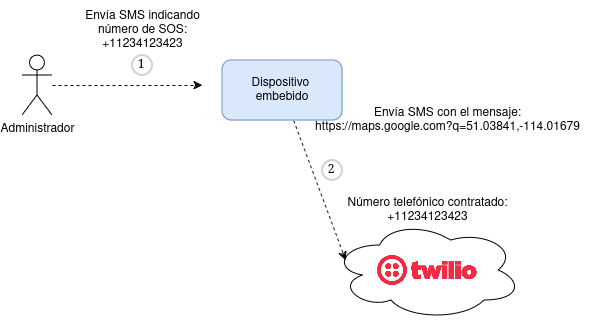
\includegraphics[width=0.9\textwidth]{./Figures/integracion-1.png}
	\caption{Esquema de integración entre botón antipánico y Twilio.}
	\label{integracion:1}
\end{figure}

Al momento de integrar el \textit{backend}, \textit{frontend}, bases de datos y servicios externos, se disponibilizó el sistema en un entorno \textit{cloud}. Los componentes web se desplegaron en la nube de Heroku mediante el uso de \textit{dynos} básicos, que son contenedores de aplicaciones web \citep{HEROKU:1}. Para la base de datos se utilizó un \textit{addon} de PostgreSQL, que consiste en un complemento que permite incorporar una base de datos como SaaS u otros componentes requeridos por los sistemas, como pueden ser bases de datos en memoria o brókers \citep{HEROKU:2}. Al momento de desplegar, fueron asignadas dos URLs, una para el \textit{frontend} y otra para la API, para permitir que el \textit{frontend} y Twilio apunten a la API correctamente.

Para la integración entre la API y Twilio, se implementó un único servicio del tipo \textit{webhook} para que se notifique en tiempo real la llegada de una nueva alerta. Para poder securizar las ejecuciones del \textit{webhook} y asegurarse de que sea ejecutado solamente por los sistemas de Twilio, se utilizó el esquema de seguridad provisto por este. Cuando Twilio realiza una petición hacia una API, incluye dos parámetros en el cuerpo de la petición \citep{TWILIO:2}:
\begin{itemize}
	\item \texttt{ACCOUNT\_SID}: identificador de la cuenta de Twilio.
	\item \texttt{AUTH\_TOKEN}: credencial para autenticación, única por cada cuenta.
\end{itemize}

Por este motivo, toda interacción debe realizarse bajo HTTPS o se corre el riesgo de que puedan filtrarse las credenciales enviadas como parámetros de la petición. El \textit{backend} utiliza estas credenciales y las compara con las credenciales configuradas como variables de configuración y determina si el originador de la llamada al \textit{webhook} es legítimo para continuar con el procesamiento. En la figura \ref{integracion:2} se puede ver la interacción entre Twilio y el \textit{backend}.

\begin{figure}[H]
	\centering
	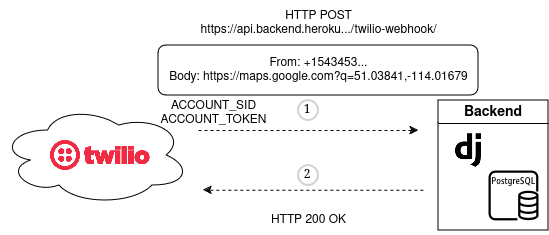
\includegraphics[width=0.9\textwidth]{./Figures/integracion-2.png}
	\caption{Esquema de integración entre Twilio y la API.}
	\label{integracion:2}
\end{figure}


Por último, en relación a la comunicación entre el \textit{frontend} del usuario y la API, toda la interacción entre el \textit{backend} y \textit{frontend} es realizada mediante \textit{endpoints} HTTP y \textit{WebSockets} para comunicación en tiempo real, utilizando TLS/SSL para securizar las conexiones. Además, para poder autorizar cada petición HTTP, el usuario debe incluir un \textit{JSON Web Token} o JWT en el encabezado de esta, que es un mensaje con formato estandarizado utilizado principalmente para autorización \citep{JWT:1}. Este token es generado por el usuario al momento de loguearse en el sistema web.

Para el caso de la conexión mediante \textit{WebSockets} o WS, usada para recibir nuevas alertas en tiempo real, se implementó otro mecanismo de autorización debido a la imposibilidad de incluir encabezados en las peticiones o conexiones. Se incorporó un \textit{endpoint} que permite que el usuario genere un token efímero de uso único para cada conexión de WS. Este token se envía como parámetro al momento de iniciar la conexión y tiene validez mientras se mantenga la conexión establecida. En la figura \ref{integracion:3} se observan los mecanismos de comunicación entre el \textit{frontend} y \textit{backend}.

\begin{figure}[H]
	\centering
	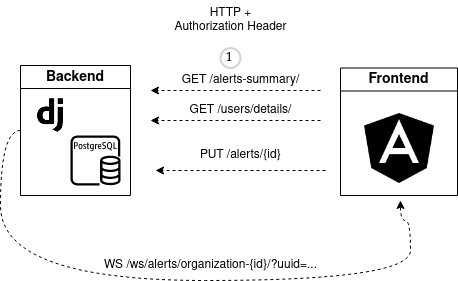
\includegraphics[width=0.8\textwidth]{./Figures/integracion-3.png}
	\caption{Esquema de integración entre \textit{frontend} y la API.}
	\label{integracion:3}
\end{figure}

